\documentclass[../report.tex]{subfiles}

\begin{document}

\subsection{Sơ lược về hệ thống phát hiện người}

\begin{figure}[H]
\centering
\includegraphics[width=\textwidth]{figures/human-detection-diagram.png}
\end{figure}

Để phát hiện một vật thể trong ảnh, 
đầu tiên cần phải huấn luyện cho hệ thống. \\
Quy trình huấn luyện \cite{hog-svm}: 
\begin{itemize}
\item Dữ liệu huấn luyện là một tập các ảnh của vật 
    thể và ảnh không chứa vật thể đã được gán nhãn 
    với nhãn 1 là ảnh vật thể, nhãn 0 là ảnh không chứa vật thể.
\item Tính đặc trưng HOG của tập ảnh. 
    Sử dụng hàm \textbf{HOGDescriptor()} trong thư viện opencv, 
    với ngôn ngữ python.
\item 
Khi đã có được tập đặc trưng HOG của các ảnh và 
nhãn tương ứng, tiến hành học phân lớp SVM với tập 
dữ liệu trên. Sử dụng hàm \textbf{svm.LinearSVC()} 
của thư viện \textbf{sklearn}. Đầu vào của hàm là mảng các đặc 
trưng HOG và nhãn tương ứng của chúng. Đầu ra là 
một vector phân lớp SVM.
\end{itemize}
Đầu vào của quá trình huấn luyện là tập các ảnh và 
nhãn tương ứng của mỗi ảnh. Đầu ra là một vector phân lớp SVM 
(hay vector tham số của mặt siêu phẳng). \\[3mm]
Quy trình phát hiện ảnh:
\begin{itemize}
    \item Đọc ảnh cần xử lý.
    \item Đưa vector phân lớp SVM vào hệ thống bằng 
        hàm \textbf{setSVMDetector()}.
    \item Tiến hành phát hiện đối tượng trong ảnh bằng 
        hàm \textbf{detectMultiScale()}.
\end{itemize}
Đầu vào của quá trình phát hiện ảnh là một ảnh. 
Đầu ra là tập vi trí các hình chữ nhật bao 
quanh đối tượng cần phát hiện.

\subsection{Ứng dụng phát hiện người}
Phát hiện người sử dụng vector được huấn luyện 
sẵn của thư viện OpenCV được lấy từ hàm 
\textbf{cv2.HOGDescriptor\_getDefaultPeopleDetector()} 
\cite{human-detection-opencv}.
Với đặc trưng HOG được tính theo bộ tham số: \\[3mm]
\begin{tabular}{|l l|}
\hline
blockSize $= (16, 16)$  &-Kích thước mỗi khối. \\
blockStride $= (8, 8)$  &-Khoảng cách giữa hai khối liền nhau.  \\
cellSize $= (8, 8)$     &-Kích thước mỗi ô. \\
nbins $= 9$             &-Số lượng tập các góc được chia. \\
\hline
\end{tabular} \\[3mm]
Dùng hàm \textbf{detectMultiScale()} 
để xác định người trong ảnh \cite{detectmultiscale-params}. \\
Với bộ tham số: \\[3mm]
\begin{tabular}{|l l|}
\hline
winStride $= (8, 8)$    &-Mức độ dịch của cửa sổ trượt. \\
scale $= 1.05$          &-Tỉ lệ thu nhỏ ảnh. \\
\hline
\end{tabular} \\[5mm]
Kết quả như hình: 
\begin{figure}[H]
\centering
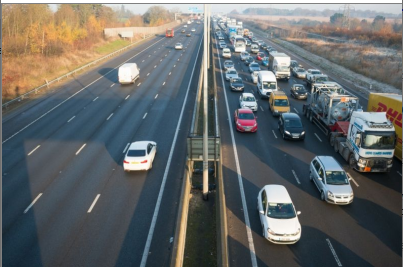
\includegraphics[width=7cm]{figures/test-1-1.png}
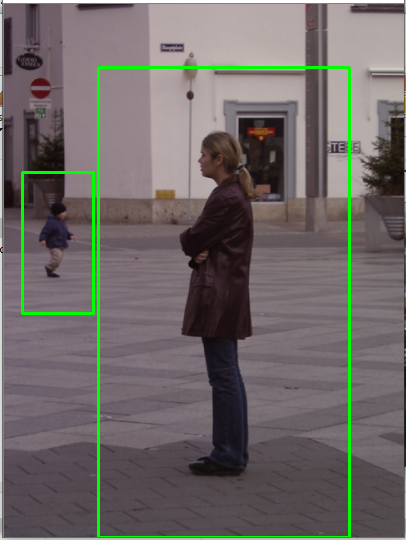
\includegraphics[width=5cm]{figures/test-1-2.png}
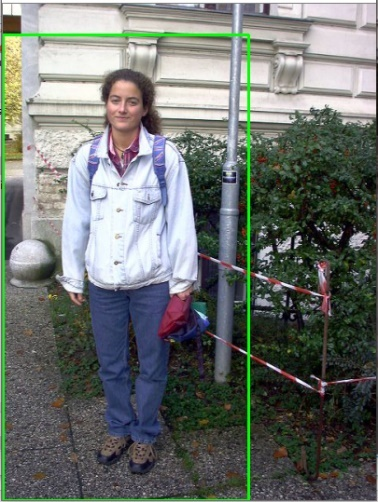
\includegraphics[width=5cm]{figures/test-1-3.png}
\end{figure}
\noindent Nếu tăng winSride $= (16,16)$ hoặc tăng  
scale lên $1.5$, thu được kết quả có sự thay đổi như hình:
\begin{figure}[H]
\centering
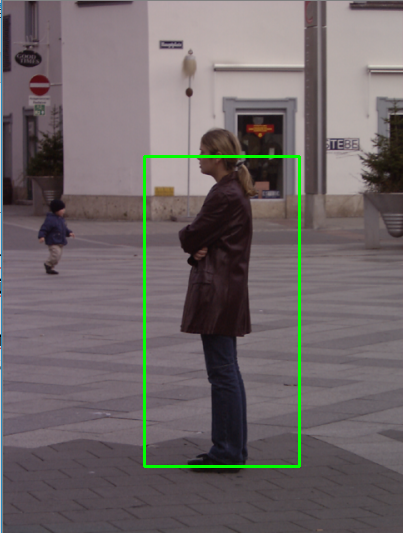
\includegraphics[width=6cm]{figures/test-2-1.png}
\end{figure}

\noindent Nhận xét:
\begin{itemize}
    \item Nếu winStride hoặc scale quá lớn, 
        một vài đối tượng sẽ bị bỏ qua – không được phát hiện.
    \item Nếu winStride hoặc scale quá nhỏ, 
        thời gian chạy thuật toán tăng lên.
\end{itemize}

\subsection{Huấn luyện phát hiện đồng hồ}
\subsubsection{Huấn luyện hệ thống}
Dữ liệu huấn luyện là tập các ảnh 
đồng hồ và không phải đồng hồ. \\[3mm]
Ảnh đồng hồ:
\begin{figure}[H]
\centering
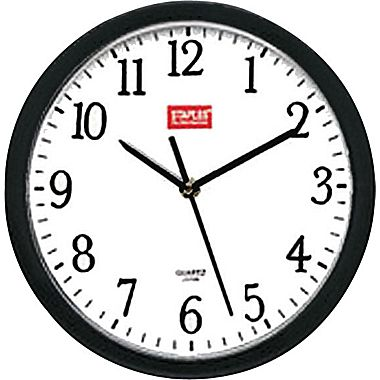
\includegraphics[width=3.5cm]{figures/clock-1.png}
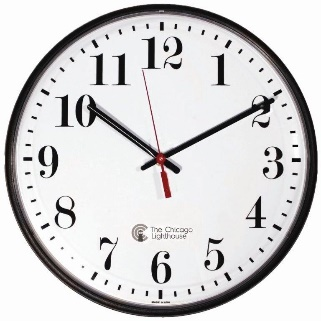
\includegraphics[width=3.5cm]{figures/clock-2.png}
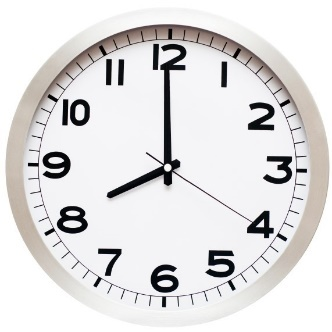
\includegraphics[width=3.5cm]{figures/clock-3.png}
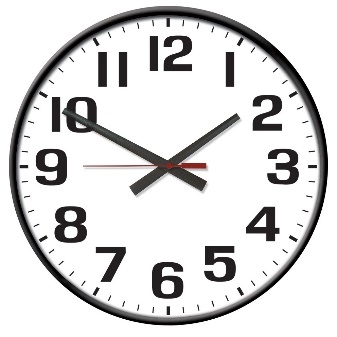
\includegraphics[width=3.5cm]{figures/clock-4.png}
\end{figure}
\noindent Ảnh không phải đồng hồ: 
\begin{figure}[H]
\centering
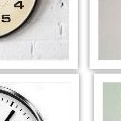
\includegraphics[width=3.5cm]{figures/nonclock-1.png}
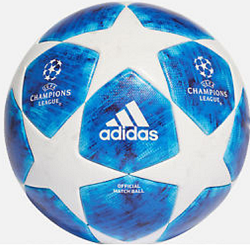
\includegraphics[width=3.5cm]{figures/nonclock-2.png}
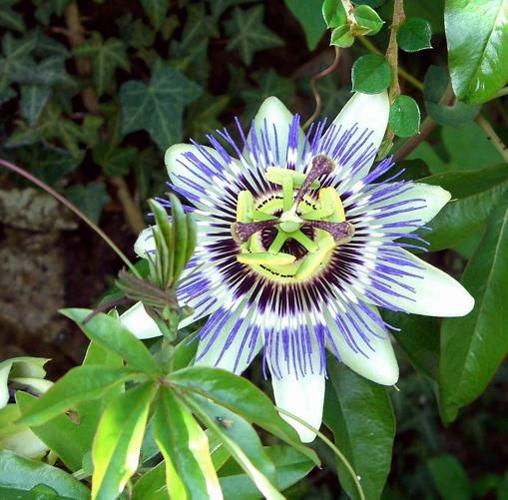
\includegraphics[width=3.5cm]{figures/nonclock-3.png}
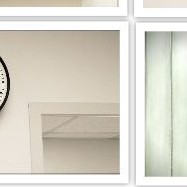
\includegraphics[width=3.5cm]{figures/nonclock-4.png}
\end{figure}
\noindent Ảnh đồng có có 55 ảnh, 
ảnh không chứa đồng hồ có 258 ảnh. \\[3mm]
Các ảnh được đưa về cùng kích thước $(64, 64)$ trước 
khi tính đặc trưng HOG và tiến hành huấn luyện mô hình.

\subsubsection{Kết quả}
Kích thước ảnh được tính HOG là $64 \times 64$. 
Với tham số tính HOG: \\[3mm]
\begin{tabular}{|l l|}
\hline
blockSize $= (16, 16)$  &-Kích thước mỗi khối. \\
blockStride $= (8, 8)$  &-Khoảng cách giữa hai khối liền nhau.  \\
cellSize $= (8, 8)$     &-Kích thước mỗi ô. \\
nbins $= 9$             &-Số lượng tập các góc được chia. \\
\hline
\end{tabular} \\[3mm]
Kết quả thu được:
\begin{figure}[H]
\centering
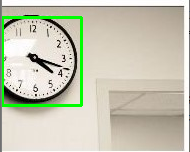
\includegraphics[width=5cm]{figures/test-3-1.png}
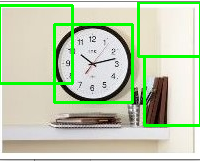
\includegraphics[width=5cm]{figures/test-3-2.png}
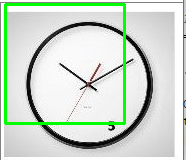
\includegraphics[width=5cm]{figures/test-3-3.png}
\end{figure}

\noindent Với tham số tính HOG: \\[3mm]
\begin{tabular}{|l l|}
\hline
blockSize $= (32, 32)$  &-Kích thước mỗi khối. \\
blockStride $= (8, 8)$  &-Khoảng cách giữa hai khối liền nhau.  \\
cellSize $= (8, 8)$     &-Kích thước mỗi ô. \\
nbins $= 9$             &-Số lượng tập các góc được chia. \\
\hline
\end{tabular} \\[3mm]
Kết quả thu được:
\begin{figure}[H]
\centering
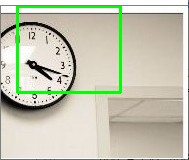
\includegraphics[width=5cm]{figures/test-4-1.png}
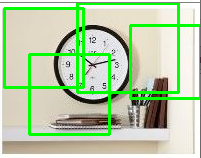
\includegraphics[width=5cm]{figures/test-4-2.png}
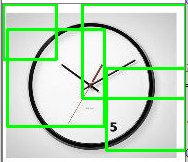
\includegraphics[width=5cm]{figures/test-4-3.png}
\end{figure}
\noindent Nhận thấy với blockSize lớn hơn, 
chương trình đưa ra nhiều ô không đúng vị trí đối tượng. \\[5mm]
Nhận xét: Chương trình chạy chưa tốt, còn phát hiện sai nhiều. 
Nguyên nhân do bộ dữ liệu huấn luyện quá nhỏ, 
không tổng quát hết được các trường hợp.

\end{document}
